% !TeX program = xelatex
% 原创讲解稿：基于用户提供的扫描教材习题 1.1，独立重新推导。
\documentclass[UTF8,a4paper,11pt,fontset=none]{ctexart}
\usepackage[margin=22mm,top=21mm,bottom=23mm,headheight=16pt,headsep=9mm]{geometry}
\setCJKmainfont{Noto Serif CJK SC}
\setCJKsansfont{Noto Sans CJK SC}
\setmainfont{Liberation Serif}
\setsansfont{Liberation Sans}
\usepackage{amsmath,amssymb,mathtools,amsthm,bm}
\usepackage{graphicx,tikz,tcolorbox,booktabs,tabularx,multirow,needspace}
\usepackage{enumitem,fancyhdr,lastpage,titlesec,xcolor,hyperref,array,multicol}
\usetikzlibrary{calc,intersections,arrows.meta}
\definecolor{navy}{HTML}{183F5D}
\definecolor{blue}{HTML}{276999}
\definecolor{light}{HTML}{EDF4F9}
\definecolor{teal}{HTML}{1A7668}
\definecolor{amber}{HTML}{986017}
\definecolor{warnbg}{HTML}{FFF5E9}
\definecolor{rulegray}{HTML}{DEE7ED}
\hypersetup{colorlinks=true,linkcolor=blue,urlcolor=blue,pdfauthor={Independent solution notes},pdftitle={空间解析几何：向量代数习题 1.1 逐题核查与详解},pdfsubject={习题答案逐题核查、重建推导、纠错与适用条件}}
\newcommand{\V}[1]{\overrightarrow{#1}}
\newcommand{\Ra}[3]{(#1,#2,#3)}
\newcommand{\R}{\mathbb R}
\newcommand{\ans}[1]{\par\noindent\textcolor{teal}{\sffamily\bfseries 核查结论：}#1\par}
\newcommand{\idea}[1]{\par\noindent\textcolor{navy}{\sffamily\bfseries 思路：}#1\par}
\newcommand{\warning}[1]{\begin{tcolorbox}[colback=warnbg,colframe=amber,boxrule=0.55pt,arc=2mm,left=3mm,right=3mm,top=2mm,bottom=2mm]\textcolor{amber}{\sffamily\bfseries 核查提醒}\quad #1\end{tcolorbox}}
\newcommand{\tip}[1]{\begin{tcolorbox}[colback=light,colframe=rulegray,boxrule=0.4pt,arc=1.5mm,left=3mm,right=3mm,top=2mm,bottom=2mm]#1\end{tcolorbox}}
\newcommand{\prob}[2]{\clearpage\phantomsection\addcontentsline{toc}{section}{第 #1 题\quad #2}\section*{第 #1 题\quad #2}\noindent\textcolor{blue}{\small 原书位置：第 1 章习题 1.1（纸质页 14--16；PDF 页 20--22）}\par\medskip}
\newcommand{\probnext}[2]{\par\Needspace{9\baselineskip}\phantomsection\addcontentsline{toc}{section}{第 #1 题\quad #2}\section*{第 #1 题\quad #2}\noindent\textcolor{blue}{\small 来源：习题 1.1，第 #1 题}\par\medskip}
\titleformat{\section}{\sffamily\Large\bfseries\color{navy}}{}{0pt}{}
\titlespacing*{\section}{0pt}{13pt}{8pt}
\setlength{\parindent}{2em}
\setlength{\parskip}{4pt}
\setlist[itemize]{leftmargin=2em,itemsep=2pt,topsep=4pt}
\setlist[enumerate]{leftmargin=2.2em,itemsep=2pt,topsep=4pt}
\allowdisplaybreaks[1]
\pagestyle{fancy}
\fancyhf{}
\fancyhead[L]{\textcolor{navy}{\footnotesize 空间解析几何 · 原创详解}}
\fancyhead[R]{\textcolor{navy}{\footnotesize 第一章 / 习题 1.1}}
\fancyfoot[L]{\textcolor{gray}{\footnotesize 版本 v1.0 · 2026-10-16}}
\fancyfoot[R]{\textcolor{gray}{\footnotesize \thepage\,/\,\pageref{LastPage}}}
\renewcommand{\headrulewidth}{0.35pt}
\renewcommand{\footrulewidth}{0pt}

% Whole-chapter layout and navigation
\hypersetup{pdftitle={空间解析几何第一章·向量代数·习题1.1至1.5逐题详解与纠错},pdfsubject={72道题逐题讲解、原书答案核查与独立勘误}}
\fancyhead[R]{\textcolor{navy}{\footnotesize 第一章 / 向量代数}}
\fancyfoot[L]{\textcolor{gray}{\footnotesize v1.1 · 2026-10-16}}
\titleformat{\subsection}{\sffamily\normalsize\bfseries\color{navy}}{}{0pt}{}
\titlespacing*{\subsection}{0pt}{13pt}{5pt}
\newcommand{\Q}[2]{\par\Needspace{8\baselineskip}\phantomsection\addcontentsline{toc}{subsection}{第 #1 题：#2}\subsection*{第 #1 题\quad #2}\vspace{-1.5mm}}
\renewcommand{\probnext}[2]{\Q{#1}{#2}}
\newcommand{\sectionlead}[4]{\noindent\begin{tcolorbox}[colback=light,colframe=rulegray,boxrule=0.45pt,arc=1.5mm,left=3mm,right=3mm,top=2mm,bottom=2mm]\small\textbf{覆盖：}#1 道题 \quad \textbf{纸质页：}#2 \quad \textbf{书后答案页：}#3\par\medskip #4\end{tcolorbox}}

\newcommand{\figcaptiontxt}[1]{\par\smallskip\noindent{\small\color{navy}\sffamily #1}\par}
\newcommand{\concepttitle}[1]{\par\smallskip\noindent{\sffamily\bfseries\color{teal}#1}\par\smallskip}


\begin{document}
\thispagestyle{empty}
\vspace*{17mm}
{\sffamily\large\color{teal}\bfseries SPATIAL ANALYTIC GEOMETRY · VERIFIED NOTES}\par
\vspace{9mm}
{\sffamily\fontsize{29}{38}\selectfont\bfseries\color{navy} 第一章 向量代数}\par
\vspace{4mm}
{\sffamily\fontsize{21}{31}\selectfont\color{blue} 习题 1.1--1.5\enspace 全章核查与详细解析}\par
\vspace{13mm}
\begin{tcolorbox}[colback=light,colframe=rulegray,arc=2mm,boxrule=0.6pt,left=5mm,right=5mm,top=5mm,bottom=5mm]
\large\textbf{72 题完整覆盖 · 从题意、方法到独立验算}\par\medskip
\normalsize
全新排版，不复制扫描页面；将\textbf{原书列出的答案／提示}与\textbf{独立推导及勘误分析}分开记录。
\begin{itemize}
\item \textbf{1.1：}23 题，仿射分比与 Ceva / Menelaus；第 5 题原题与书后答案矛盾。
\item \textbf{1.2：}10 题，仿射坐标、坐标变换、共面 / 共线判别。
\item \textbf{1.3：}14 题，长度、投影、内积恒等式。
\item \textbf{1.4：}11 题，右手定向、面积、外积恒等式。
\item \textbf{1.5：}14 题，混合积、二重外积；第 2 题印刷公式疑缺平方，第 5(2) 题左手坐标的符号待勘误。
\end{itemize}
\end{tcolorbox}
\vfill
{\small\noindent\textbf{题源：}用户提供的 318 页《空间解析几何》扫描材料；第一章题目为纸质页 14--46（PDF 20--52），习题答案为纸质页 294--296（PDF 300--302）。\par}
{\small\noindent\textbf{形式：}原创学习解题讲义 · A4 可搜索文字 · 目录可跳转 · XeLaTeX 源码可复现。\par}
{\footnotesize\color{gray}请注意：资料并非出版社正式勘误表；标注“疑误”的地方均附数学证据及适用假设。公开发布请勿上传原始扫描件。}\par
\clearpage
\begin{multicols}{2}
\footnotesize\setlength{\parskip}{0pt}\tableofcontents
\end{multicols}
\clearpage
\section*{全章阅读说明与答案核查索引}
\addcontentsline{toc}{section}{阅读说明与核查索引}
\noindent\textbf{计算口径：}向量的坐标按题给仿射基分解，必要时另选直角正交基；直角系的左／右手方向对三重积符号有影响。\\
\textbf{有向分比：}设三点 $A,B,P$ 共线，$P=A+t(B-A)$，则
\begin{equation}\label{eq:ratio}
(A,B,P)=\frac{t}{1-t},\qquad
P=\frac{A+\lambda B}{1+\lambda}\quad(\lambda=(A,B,P)).
\end{equation}
分母为零的端点需单独处理；三点一线与三向量共面不能混为一谈。
\par\smallskip\par\noindent\begin{tabularx}{\linewidth}{@{}p{17mm}p{35mm}X@{}}\toprule
节次 & 书后列值／提示 & 核查结论与关注点\\\midrule
1.1 & 部分题目 & 23/23 详解；第 5 题向量方向矛盾；第 22 题延长线平行例外。\\
1.2 & 1--6、10 & 10/10 详解；书后列数值均独立核对。\\
1.3 & 1--7、13--14 & 14/14 详解；第 6(4) 补充零系数情况。\\
1.4 & 1--3、8--11 & 11/11 详解；第 11 题解释锐角选取。\\
1.5 & 3--6、13--14 & 14/14 详解；第 2 题分母疑误；第 5(2) 左手系定向存在符号差异。\\\bottomrule
\end{tabularx}\par\medskip
\tip{\textbf{状态说明：}“原书一致”仅用于扫描答案页确实列出且重新核对过的结果；“独立证明”表示原书未给终值，或只列提示。复杂证明中的每个判断均写明假设，不将自动测试当作对所有命题的形式化证明。}
\clearpage
\section{习题 1.1：向量的线性运算}\label{sec:11}
\sectionlead{23}{14--16}{300}{向量的加、减、数乘、重心、仿射相关与有向分比。保留原有独立核查结论和详解；尤其注意书后答案与题干不一致的第 5 题。}
\begin{tcolorbox}[colback=white,colframe=rulegray,boxrule=0.4pt,arc=1.5mm,left=2mm,right=2mm,top=1.5mm,bottom=1.5mm]
\concepttitle{图形理解 1.1：线段分点与三角形中的共点 / 共线}
\begin{minipage}[t]{0.47\linewidth}
\centering
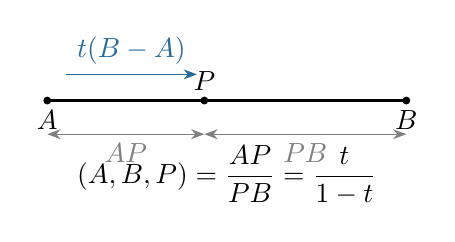
\begin{tikzpicture}[scale=0.95,>=Stealth]
\coordinate (A) at (0,0);
\coordinate (B) at (4.8,0);
\coordinate (P) at (2.1,0);
\draw[thick] (A)--(B);
\fill (A) circle(1.5pt) node[below]{$A$};
\fill (P) circle(1.5pt) node[above]{$P$};
\fill (B) circle(1.5pt) node[below]{$B$};
\draw[->,blue] (0.25,0.35)--(2.0,0.35) node[midway,above]{$t(B-A)$};
\draw[<->,gray] (0,-0.45)--(2.1,-0.45) node[midway,below]{$AP$};
\draw[<->,gray] (2.1,-0.45)--(4.8,-0.45) node[midway,below]{$PB$};
\node at (2.4,-1.0) {$(A,B,P)=\dfrac{AP}{PB}=\dfrac{t}{1-t}$};
\end{tikzpicture}
\figcaptiontxt{同一直线上用参数 $P=A+t(B-A)$ 最稳妥；一旦写出 $t$，有向分比、内分外分就都统一了。}
\end{minipage}\hfill
\begin{minipage}[t]{0.49\linewidth}
\centering
\begin{tikzpicture}[scale=0.95,>=Stealth]
\coordinate (A) at (0.2,0.1);
\coordinate (B) at (3.8,0.1);
\coordinate (C) at (1.4,2.8);
\coordinate (D) at ($(B)!0.42!(C)$);
\coordinate (E) at ($(C)!0.50!(A)$);
\coordinate (F) at ($(A)!0.58!(B)$);
\coordinate (O) at (1.8,1.15);
\draw[thick] (A)--(B)--(C)--cycle;
\draw[blue] (A)--(D);
\draw[blue] (B)--(E);
\draw[blue] (C)--(F);
\fill (A) circle(1.3pt) node[below]{$A$};
\fill (B) circle(1.3pt) node[below]{$B$};
\fill (C) circle(1.3pt) node[above]{$C$};
\fill (D) circle(1.3pt) node[right]{$D$};
\fill (E) circle(1.3pt) node[left]{$E$};
\fill (F) circle(1.3pt) node[below]{$F$};
\fill[red] (O) circle(1.5pt) node[right]{$O$};
\node at (2.0,-0.65) {Ceva / Menelaus 常靠“边上分点 + 乘积关系”判断};
\end{tikzpicture}
\figcaptiontxt{第 22、23 题可先看成“边上的分点是否让三条线共点 / 三点共线”，再上公式。}
\end{minipage}
\end{tcolorbox}
\input{chapters/01-01-body.tex}
\clearpage
\input{chapters/01-02.tex}
\clearpage
\input{chapters/01-03.tex}
\clearpage
\input{chapters/01-04.tex}
\clearpage
\input{chapters/01-05.tex}
\clearpage
\section*{全章勘误与复习清单}\addcontentsline{toc}{section}{全章勘误与复习清单}
\begin{enumerate}
\item \textbf{疑误 A（习题 1.1 第 5 题）：}题干 $\V{DE}=\alpha$ 与书后答案所暗含的 $\V{DE}=-\alpha$ 不相容；本讲义保留两种条件的比较，不擅自声称官方勘误。
\item \textbf{疑误 B（习题 1.5 第 2 题）：}分母印为 $|\alpha|$，BAC--CAB 推导要求分母是 $|\alpha|^2$；若 $\alpha$ 不是单位向量，原等式通常不成立。
\item \textbf{疑误 C（习题 1.5 第 5(2) 题）：}书后给 $+36$，但若外积固定使用通常的右手定向，则左手直角坐标中有向混合积为 $-36$。请结合课本对混合积和定向的正式定义确认。
\item \textbf{适用条件（习题 1.1 第 22 题）：}Ceva 的乘积关系延长线情形可能出现三线平行，需要分情况判断有限共点。
\end{enumerate}
\tip{\textbf{复习建议：}先记住 $\alpha\cdot\beta=|\alpha||\beta|\cos\theta$、$|\alpha\times\beta|=|\alpha||\beta|\sin\theta$ 与 BAC--CAB；做题依次判断坐标系、端点次序、是否非零／不共线，再开始运算。}
\vspace{3mm}
\noindent{\small\textbf{版本：}v1.1，2026-10-16。对应可重复构建的 LaTeX 源码与 SymPy 核查脚本。题目使用概要重述和自主推导，既便于学习也便于 GitHub 维护。}
\end{document}
